\subsection{True-Velocity Randomized Paths}
We separately probe the reversible randomized torus path in \cref{eq:noisy-torus} on General, with $\varepsilon\in\{0,0.3,0.7\}$. The actual derivative includes the noise-amplitude derivative. The experiment uses a randomly initialized MLP, the periodic critic, seed 0, batch 512, 10,000 generator updates, five critic updates per generator step, 500 critic warmup updates, and generator/critic learning rates $2\times10^{-4}$. All three amplitudes and fixed checkpoints are specified before this diagnostic. It is post hoc validation-only evidence, not a replacement for the primary table or independent-seed confirmation. Evaluation preserves the training RNG state.
Table~\ref{tab:noise} lists every amplitude. Figure~\ref{fig:noise} shows the fixed-checkpoint validation curves. The $\varepsilon=0$ row is a separately executed deterministic control with the same code path and random draws, not a copied earlier result.
\begin{table}[t]\caption{Randomized-torus validation diagnostic. One seed-0 model per amplitude; MMD$^2\times10^3$ means average three sampling draws. The final SD is Monte Carlo variation only. No test metrics are evaluated.}\label{tab:noise}\centering\small\begin{tabular}{@{}rrrrr@{}}\toprule
Amplitude $\varepsilon$ & Initial val. & Final val. & Final MC SD & Train s \\
\midrule
0 & 750.34 & 60.70 & 3.86 & 159.9 \\
0.3 & 750.34 & 36.53 & 1.85 & 156.0 \\
0.7 & 750.34 & 31.68 & 0.71 & 150.2 \\
\bottomrule\end{tabular}\end{table}
Noise improves the final validation MMD relative to this deterministic control in the single-seed sweep, but all three models remain above the periodic RFM reference (approximately $1.91\times10^{-3}$). Their 60,500 total optimizer updates exceed that reference's 22,500 field updates; neither update counts nor FLOPs are matched. This diagnostic does not establish cross-seed efficacy or an advantage over the flow.
\begin{figure}[t]\centering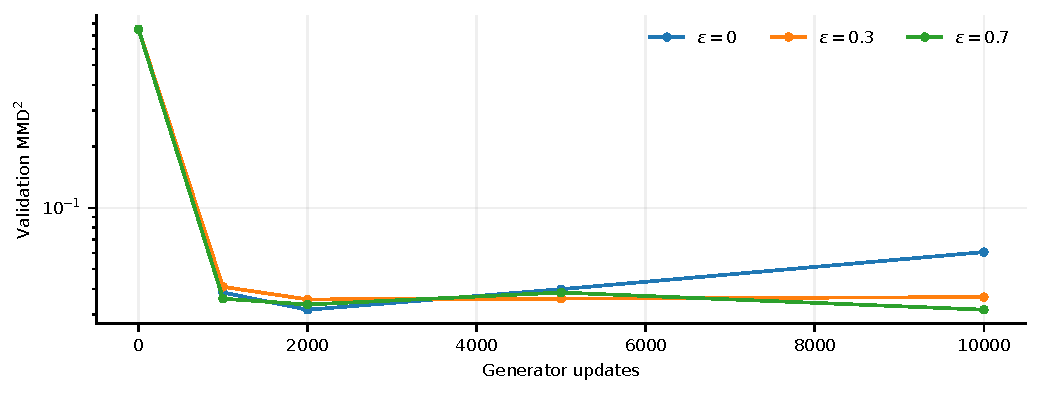
\includegraphics[width=\textwidth]{figures/validation_noise.pdf}
\caption{Validation-only true-velocity noise diagnostic. Lines join prespecified checkpoints for three seed-0 models. Different amplitudes define different path discrepancies; these curves do not estimate the population divergence or establish a generally optimal noise level.}\label{fig:noise}\end{figure}
